% !TEX root = ../main.tex
\chapter{PCSEL 的半导体外延层与纵向光学结构}
\label{ch:epitaxial-optics}

\section*{学习目标}
\begin{itemize}
  \item 理解为什么在 PCSEL 中，外延层不是平面内光子晶体的背景板，而是与晶格设计并列的第一性器件变量。
  \item 掌握分离限制异质结构（separate confinement heterostructure, SCH）、异质结和能带对齐怎样同时进入纵向光学约束与后续电注入设计。
  \item 能够把纵向波导模式、量子阱重叠、损耗层重叠、上下辐射不对称和材料台阶设计放到同一条器件链上理解。
\end{itemize}

\section*{先修知识}
建议已掌握 \cref{ch:feedback,ch:threshold,ch:method-compare} 中关于面发射、阈值损耗、开放系统与数值方法分工的内容。

\section*{本章路线图}
\ChapterModelLevel{L2}
\crefrange{ch:bloch}{ch:method-compare} 把 PCSEL 当作周期开放电磁系统来理解，并已经得到一套关于候选模、辐射损耗、阈值增益和数值工作流的语言。但真实器件不会把这些结论“原封不动”交给实验，因为真正工作的模式并不生活在抽象二维平面里，而是嵌入在异质结外延层、量子阱、有损接触层和非对称边界条件共同构成的纵向结构中。本章的任务，就是把这条纵向主线搭起来。我们先回答为什么 PCSEL 必须采用分离限制异质结构，再说明导带、价带台阶如何进入设计；随后把典型层栈、纵向波导、本征模、有效折射率近似、重叠积分与损耗重叠放到一条链上，最后解释为什么这些外延细节会直接改写前面章节得到的冷腔排序与远场判断。

\section{从二维光子晶体到真实器件：缺的不是一层材料，而是一整条纵向物理链}
如果只顺着前面的 Maxwell、Bloch、CWT 和全波仿真章节读下来，读者很容易形成一种危险印象：仿佛 PCSEL 的主要设计自由度都在平面内，外延层只是“把这个结构长出来”的工艺载体。这在真实器件层面是错误的。原因很直接，前面得到的一切候选模、辐射耦合、Gamma 点排序和阈值增益需求，最终都要投影到一个实际三维模式上；而三维模式的纵向位置、与量子阱的重叠、与掺杂层和金属的重叠、对上/下辐射通道的耦合，全部由外延层决定。

换句话说，前面章节回答的是“如果给定一个纵向背景，平面内周期结构会如何组织反馈和辐射”；本章开始回答的是“这个纵向背景本身应该如何被搭建，才能让前面那些冷腔结论在真实器件里仍然有意义”。这也是为什么本书反复提醒：PCSEL 不是普通光子晶体共振器。只要进入器件层面，纵向外延结构就和二维晶格一样，都是模式选择的一部分。

\begin{IntuitionBox}
平面内晶格决定的是“面内波如何耦合、怎样辐射到法向”；外延层决定的是“这些波被束缚在什么高度、穿过哪些层、与哪些损耗区和有源区重叠”。前者给出反馈图样，后者决定这张图样能否成为真正的器件模式。
\end{IntuitionBox}

\section[SCH 与器件可行性]{为什么 PCSEL 几乎总要落到 SCH：分离限制异质结构不是教科书惯例，而是器件可行性的起点}
分离限制异质结构（SCH）的核心思想，是把“强光学场区域”和“主要载流子受限区域”通过异质材料台阶组织在一起，但又不把两者机械地做成同一层。更具体地说，量子阱区负责提供受激辐射增益，周围较低折射率但带隙更大的波导/限制层负责把模式束缚在量子阱附近，同时提供载流子的势垒环境。这种“有源区很薄、光学模更宽、两者通过重叠而非完全重合来耦合”的结构，就是现代半导体激光器和 PCSEL 中最常见的纵向架构。

为什么 PCSEL 尤其需要 SCH？原因至少有三条。

第一，如果把增益材料本身直接做成唯一波导层，模式会过于贴近高吸收、高散射或高掺杂区域，阈值增益需求迅速恶化。第二，PCSEL 常常还需要在量子阱上方再放入光子晶体层、接触层乃至空气孔结构，这要求光学模既要与量子阱有足够重叠，又不能被过度拉向表面损耗区。第三，面发射器件中上下边界天然不对称，如果没有 SCH 提供的纵向缓冲和再分配空间，模式很容易被上表面工艺层或下方衬底通道拖偏。

因此，SCH 不是“传统边发射激光器也这么做，所以 PCSEL 也顺便照搬”的结构模板，而是把 \cref{ch:threshold} 的阈值条件真正放进器件里时最基本的器件逻辑：它让模式可以在量子阱附近获得足够光学重叠，又不至于被表面与接触损耗吃掉。
为了帮助读者直观理解 PCSEL 的典型纵向外延层堆叠结构，\cref{fig:ch16_epitaxial_stack}展示了一个完整的 GaAs 基 PCSEL 外延层结构示意图，从下至上依次包括：GaAs 衬底、n-DBR反射镜（20-30对AlGaAs异质结）、下SCH波导层（约200 nm）、多量子阱有源区（3-5个InGaAs阱）、上SCH波导层（约200 nm）、光子晶体层、电流阻挡层和 p型接触层。图中清晰标注了各层的典型厚度范围、材料体系和掺杂类型，这些参数对于理解后续章节的电注入设计和热管理策略至关重要。

% !TEX root = ../main.tex
% Figure: Epitaxial stack cross-section with layer functions
% Chapter: ch16 - Epitaxial and Optical Structure Design
% Description: Complete vertical structure of a typical PCSEL

\begin{figure}[htbp]
  \centering
  \begin{tikzpicture}[scale=1.0]
    % Substrate at bottom
    \fill[gray!40] (-3,-5) rectangle (3,-4);
    \draw[thick] (-3,-4) -- (3,-4);
    \node[right] at (3.1,-4.5) {GaAs 衬底 ($n$-doped)};
    \node[left, gray!60] at (-3,-4.5) {\scriptsize $500\,\mu\mathrm{m}$};
    
    % Lower DBR mirror
    \foreach \i in {0,...,7} {
      \pgfmathparse{\i*0.3-3.8}
      \fill[blue!\the\numexpr\i*10!green!60!black!20] (-3,\pgfmathresult) rectangle (3,{\pgfmathresult+0.15});
      \draw[thin, gray] (-3,\pgfmathresult) -- (3,\pgfmathresult);
    }
    \draw[thick] (-3,-3.8) -- (3,-3.8);
    \node[right] at (3.1,-3.5) {$n$-DBR (20--30 对)};
    \node[left, blue] at (-3,-3.5) {\scriptsize Al$_{0.9}$Ga$_{0.1}$As/Al$_{0.2}$Ga$_{0.8}$As};
    
    % Lower SCH waveguide
    \fill[green!15] (-3,-3.2) rectangle (3,-2.5);
    \draw[thick] (-3,-3.2) -- (3,-3.2);
    \draw[thick] (-3,-2.5) -- (3,-2.5);
    \node[right] at (3.1,-2.85) {下 SCH 波导层};
    \node[left, green!60!black] at (-3,-2.85) {\scriptsize $200\,\mathrm{nm}$};
    
    % Active region (MQW)
    \fill[red!20] (-3,-2.5) rectangle (3,-2.2);
    \draw[thick] (-3,-2.5) -- (3,-2.5);
    % Quantum wells inside active region
    \foreach \y in {-2.45,-2.35,-2.25} {
      \fill[red!60] (-3,\y) rectangle (3,{\y+0.05});
      \draw[dashed, red] (-3,\y) -- (3,\y);
    }
    \draw[thick] (-3,-2.2) -- (3,-2.2);
    \node[right] at (3.1,-2.35) {有源区 (3--5 阱 MQW)};
    \node[left, red] at (-3,-2.35) {\scriptsize In$_{0.2}$Ga$_{0.8}$As};
    
    % Upper SCH waveguide
    \fill[green!15] (-3,-2.2) rectangle (3,-1.5);
    \draw[thick] (-3,-2.2) -- (3,-2.2);
    \draw[thick] (-3,-1.5) -- (3,-1.5);
    \node[right] at (3.1,-1.85) {上 SCH 波导层};
    \node[left, green!60!black] at (-3,-1.85) {\scriptsize $200\,\mathrm{nm}$};
    
    % Photonic crystal layer
    \fill[yellow!30] (-3,-1.5) rectangle (3,-0.8);
    \draw[thick] (-3,-1.5) -- (3,-1.5);
    % Etched holes
    \foreach \x in {-2.5,-1.5,...,2.5} {
      \fill[white] (\x,-1.15) circle (0.15);
      \draw[thick] (\x,-1.15) circle (0.15);
    }
    \draw[thick] (-3,-0.8) -- (3,-0.8);
    \node[right] at (3.1,-1.15) {PhC 光栅层 (刻蚀深度~$150\,\mathrm{nm}$)};
    \node[left, yellow!60!black] at (-3,-1.15) {\scriptsize $\Lambda=260\,\mathrm{nm}$};
    
    % Upper cladding / contact
    \fill[orange!20] (-3,-0.8) rectangle (3,-0.3);
    \draw[thick] (-3,-0.8) -- (3,-0.8);
    \draw[thick] (-3,-0.3) -- (3,-0.3);
    \node[right] at (3.1,-0.55) {$p$-AlGaAs 包层};
    \node[left, orange] at (-3,-0.55) {\scriptsize $500\,\mathrm{nm}$};
    
    % Contact metal
    \fill[gray!60] (-3,-0.3) rectangle (3,0);
    \draw[thick] (-3,-0.3) -- (3,-0.3);
    \draw[thick] (-3,0) -- (3,0);
    \node[right] at (3.1,-0.15) {$p$-接触电极 (Ti/Pt/Au)};
    \node[left, gray] at (-3,-0.15) {\scriptsize $200\,\mathrm{nm}$};
    
    % Bonding layer (optional)
    \fill[purple!20] (-3,0) rectangle (3,0.3);
    \draw[thick] (-3,0) -- (3,0);
    \draw[thick] (-3,0.3) -- (3,0.3);
    \node[right] at (3.1,0.15) {键合层 (Au-Sn/$\mathrm{SiO_2}$)};
    \node[left, purple] at (-3,0.15) {\scriptsize 倒装焊可选};
    
    % Heat sink at top
    \fill[cyan!30] (-3,0.3) rectangle (3,1);
    \draw[thick] (-3,0.3) -- (3,0.3);
    \draw[thick] (-3,1) -- (3,1);
    \node[right] at (3.1,0.65) {热沉 (Cu/W 或金刚石)};
    \node[left, cyan!60!black] at (-3,0.65) {\scriptsize 高热导率};
    
    % Current flow arrows
    \draw[->, very thick, red] (-4,-0.15) -- node[left] {$I_{inj}$} (-4,-3.5);
    
    % Light emission arrow
    \draw[->, very thick, green!60!black] (0,-0.8) -- (0,1.5);
    \node[right, green!60!black, font=\bfseries] at (0.2,1.2) {激光输出};
    
    % Total thickness bracket
    \draw[thick] (3.5,-4) -- node[right] {外延总厚~$8$--$12\,\mu\mathrm{m}$} (3.5,0.3);
    
    % Mode profile overlay (schematic)
    \draw[very thick, blue, opacity=0.5, domain=-3:3, samples=100] 
      plot(\x,{0.3*cos(deg(0.5*\x))*exp(-(\x+0.5)*(\x+0.5)/4)-1.85});
    \node[blue, align=center] at (2,-1.5) {基模场分布\\$\mathrm{LP}_{01}$};
  \end{tikzpicture}
  \caption{典型 PCSEL 外延堆栈的截面示意图（未按比例）。图中依次给出衬底、DBR、上下 SCH 波导层、有源量子阱区、光子晶体层、包层与金属接触，并标出注入电流方向、垂直出光方向以及基模近场包络。右侧括号给出总外延厚度的典型量级。}
  \label{fig:ch16_epitaxial_stack}
\end{figure}

\section{异质结和能带对齐为什么必须在本章就讲}
如果只把本章理解成“光学层栈设计”，容易以为能带对齐属于后面电学章节。但这会把问题人为切断。异质结一方面通过折射率台阶形成光学波导，另一方面又通过带隙差形成载流子势垒；这两种作用来自同一组材料选择，因此必须在本章同时建立直觉。

设量子阱或波导层与限制层之间的带隙差为
\begin{equation}
\Delta E_g = E_{g,\mathrm{barrier}} - E_{g,\mathrm{well}},
\end{equation}
则工程上常把它分解为导带与价带台阶
\begin{equation}
\Delta E_c = Q_c \Delta E_g,
\qquad
\Delta E_v = (1-Q_c)\Delta E_g,
\label{eq:band_offsets}
\end{equation}
其中 $Q_c$ 是导带偏移系数。\cref{eq:band_offsets} 属于\textbf{器件材料与电学-光学接口模型}。它的意义在于：材料层一旦确定，不仅折射率剖面确定了，电子与空穴在纵向上看到的势垒也同时确定了。

对常见 III--V 体系，$Q_c$ 往往落在 $0.3$--$0.7$ 的范围内；教材级估算时，GaAs/AlGaAs 常可先取 $Q_c\approx0.67$（室温 $T\approx300\,\mathrm{K}$ 值，高温下因热膨胀和形变势变化会有漂移，高功率 PCSEL 分析时需重新校准），InGaAsP/InP 常取 $Q_c\approx0.35$--$0.40$，而 InGaN/GaN 体系由于极化场、应变和组分敏感性更强，常只能把 $Q_c\approx0.7$ 视为起始量级而非定值。这里最重要的不是背一个”标准值”，而是记住它只是\textbf{材料平台相关的分配系数}，不是普适常数。只要 $Q_c$ 变化，电子与空穴各自的限制强弱、泄漏倾向以及对阻挡层的需求都会一起改变。

这对 PCSEL 的影响非常直接。若 $\Delta E_c$ 太小，电子在高注入或高温下容易越过量子阱区泄漏到上包层或接触层；若 $\Delta E_v$ 太小，则空穴更难被有效限制在有源区，因为空穴有效质量更大、迁移率更低、注入路径也常更差。于是，一个看似“光学上模重叠不错”的外延层，只要能带台阶设计不合理，到了电注入时就会表现出电子泄漏、空穴堆积或有源区载流子不足。这正是“冷腔结论不能直接变成器件结论”的第一层原因。

\begin{figure}[htbp]
  \centering
  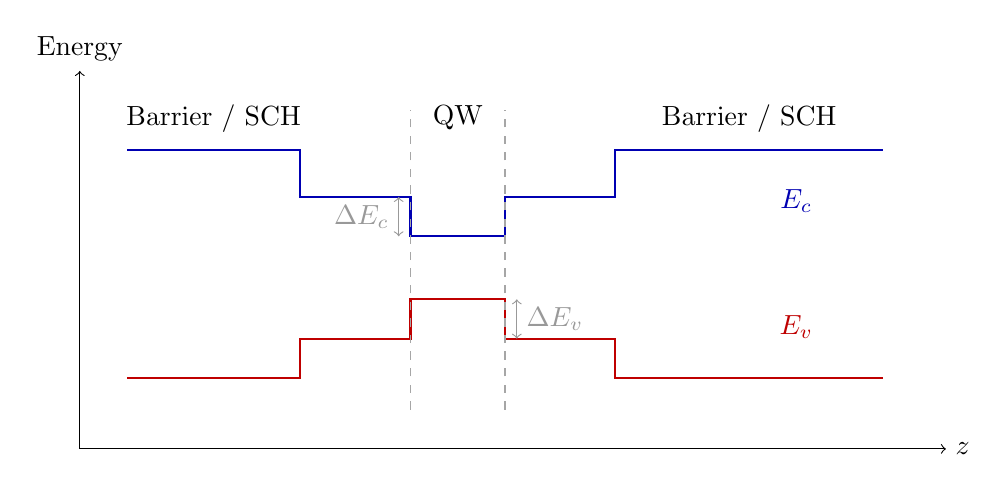
\begin{tikzpicture}[x=1cm,y=1cm]
    \draw[->] (0,0) -- (11,0) node[right] {$z$};
    \draw[->] (0,0) -- (0,4.8) node[above] {Energy};
    \draw[thick,blue!70!black]
      (0.6,3.8) -- (2.8,3.8) -- (2.8,3.2) -- (4.2,3.2) -- (4.2,2.7) -- (5.4,2.7)
      -- (5.4,3.2) -- (6.8,3.2) -- (6.8,3.8) -- (10.2,3.8);
    \draw[thick,red!75!black]
      (0.6,0.9) -- (2.8,0.9) -- (2.8,1.4) -- (4.2,1.4) -- (4.2,1.9) -- (5.4,1.9)
      -- (5.4,1.4) -- (6.8,1.4) -- (6.8,0.9) -- (10.2,0.9);
    \draw[dashed,gray!70] (4.2,0.5) -- (4.2,4.3);
    \draw[dashed,gray!70] (5.4,0.5) -- (5.4,4.3);
    \node at (1.7,4.2) {Barrier / SCH};
    \node at (4.8,4.2) {QW};
    \node at (8.5,4.2) {Barrier / SCH};
    \node[blue!70!black] at (9.1,3.15) {$E_c$};
    \node[red!75!black] at (9.1,1.55) {$E_v$};
    \draw[<->,gray!80] (4.05,3.2) -- node[left] {$\Delta E_c$} (4.05,2.7);
    \draw[<->,gray!80] (5.55,1.4) -- node[right] {$\Delta E_v$} (5.55,1.9);
  \end{tikzpicture}
  \caption{量子阱与限制层的导带/价带台阶示意。对 PCSEL 来说，这些台阶既决定载流子限制，也通过材料选择间接决定纵向折射率结构。}
  \label{fig:sch-band-offset}
\end{figure}

对电注入 PCSEL 来说，还应把这张图读成一个位置关系示意：MQW 有源区通常埋在波导/SCH 区内，而光子晶体层多位于其上方的上波导或近表面区域。这样设计的目的不是让量子阱本身被直接刻蚀，而是让目标纵模的倏逝尾既能取样光子晶体散射，又保留对 MQW 的较高重叠与较低工艺损伤风险。

\section{电子泄漏和空穴注入困难为什么会在 PCSEL 中显得更尖锐}
在很多边发射激光器教材中，电子泄漏和空穴注入困难已经是标准话题；PCSEL 并没有逃离这些问题，反而因为大面积器件和上表面结构复杂性，常常更敏感。其根本原因是：PCSEL 不是只要求“局部有增益”，而是要求在较大横向区域内形成与目标模式匹配的有效模增益分布。任何纵向泄漏机制都会把这种大面积匹配打碎。

电子泄漏通常在两种情况下变严重：一是导带势垒不够高，二是有源区上方电场和温度抬高后，电子更容易跨越势垒进入上包层、接触层甚至表面附近高损耗区域。空穴注入困难则来自另一个方向：空穴迁移率较低、有效质量较大，且在很多材料体系中可用的价带势垒工程窗口更窄，于是空穴更容易在 p 侧波导区或限制层累积，而不是均匀进入所有量子阱。结果就是：从电流看来已经“打进去了”，从增益看来却没有真正把有源区均匀填满。

对于 PCSEL，这些机制之所以必须提前讲，是因为它们最终会把 \cref{ch:qw-gain} 的材料增益和 \cref{ch:electrical} 的注入分布改写成一个横向、纵向都不均匀的器件工作点。前面章节的冷腔模式排序，到了这里就开始遇到真正的器件反例。

\begin{RigorousBox}
异质结的带边台阶不只是输运章节的输入参数，也不只是材料生长的工艺结果。它们从一开始就在回答一个器件级问题：在保证目标模式纵向光学重叠的同时，是否还能把电子和空穴真正限制在有源区附近。若这两件事不能同时成立，那么高 $Q$、高重叠或漂亮远场都不会自动变成低阈值器件。
\end{RigorousBox}

\section{典型 PCSEL 外延层从下到上分别承担什么角色}
现在再回到层栈本身。对于典型电注入 PCSEL，自下而上常见的层包括：衬底、下包层、下 SCH/波导层、量子阱区、上 SCH/波导层、光子晶体层、上包层、扩展/接触层与金属。不同路线还可能加入隧穿结、电流阻挡层、电子阻挡层或单独的 current spreading layer。它们的作用不能只按材料名记忆，而应按“对模式、载流子与损耗分别做了什么”来理解。

衬底与下包层主要提供机械支撑、散热通道和下方折射率边界；上下 SCH/波导层把模式缓慢引导到量子阱附近，同时给异质结台阶留出设计空间；量子阱区负责提供受激辐射增益；光子晶体层既参与平面内反馈，也会重新分配纵向模剖面；上包层、接触层与金属则在保证注入的同时引入自由载流子吸收、金属吸收和表面工艺约束。

最关键的是，这些层并不是先后无关的功能拼接，而是一个耦合系统。比如为了降低串联电阻而加厚上接触层，可能让模式尾部更靠近高损耗区；为了提高表面耦合而把光子晶体层放得更靠近量子阱，又可能让刻蚀损伤和表面复合风险上升。外延设计从一开始就是多目标平衡，而不是“先光学、后电学”。

\begin{figure}[htbp]
  \centering
  \resizebox{0.88\textwidth}{!}{%
  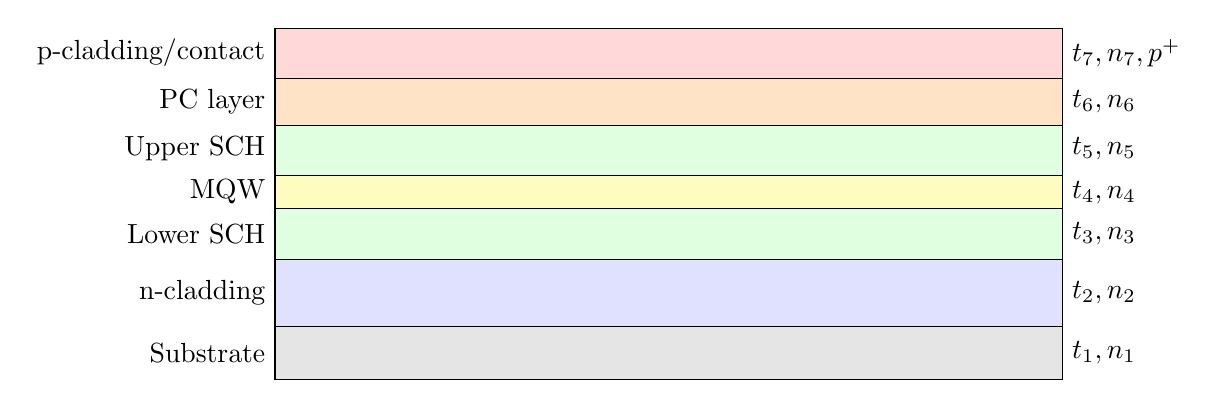
\begin{tikzpicture}[x=1cm,y=0.85cm]
    \draw[fill=gray!20] (0,0) rectangle (10,0.8);
    \draw[fill=blue!12] (0,0.8) rectangle (10,1.8);
    \draw[fill=green!12] (0,1.8) rectangle (10,2.55);
    \draw[fill=yellow!25] (0,2.55) rectangle (10,3.05);
    \draw[fill=green!12] (0,3.05) rectangle (10,3.8);
    \draw[fill=orange!22] (0,3.8) rectangle (10,4.5);
    \draw[fill=red!15] (0,4.5) rectangle (10,5.25);
    \node[left] at (0,0.4) {Substrate};
    \node[left] at (0,1.3) {n-cladding};
    \node[left] at (0,2.18) {Lower SCH};
    \node[left] at (0,2.8) {MQW};
    \node[left] at (0,3.45) {Upper SCH};
    \node[left] at (0,4.15) {PC layer};
    \node[left] at (0,4.88) {p-cladding/contact};
    \node[right] at (10,0.4) {$t_1,n_1$};
    \node[right] at (10,1.3) {$t_2,n_2$};
    \node[right] at (10,2.18) {$t_3,n_3$};
    \node[right] at (10,2.8) {$t_4,n_4$};
    \node[right] at (10,3.45) {$t_5,n_5$};
    \node[right] at (10,4.15) {$t_6,n_6$};
    \node[right] at (10,4.88) {$t_7,n_7,p^+$};
  \end{tikzpicture}
  }
  \caption{典型 PCSEL 外延层纵向结构示意。真正重要的不是材料名录，而是每一层怎样同时参与光学约束、载流子限制和损耗分布。}
  \label{fig:epi-stack}
\end{figure}

\section{从 slab 波导方程开始理解纵向模式}
一旦把平面内周期调制暂时冻结，PCSEL 的纵向问题首先就是一个层状波导问题。若只考虑沿 $z$ 方向变化的折射率剖面 $n(z)$，则在标量近似下可写
\begin{equation}
\frac{\dd^2\psi}{\dd z^2} + k_0^2 n^2(z)\psi - \betaslab^2 \psi = 0,
\label{eq:slab_waveguide}
\end{equation}
其中 $\psi(z)$ 为纵向模剖面，$\betaslab$ 为面内传播常数，$k_0=\omega/c$。这里统一用下标写成 $\betaslab$，避免与噪声章节的 $\betasp$ 混淆。\cref{eq:slab_waveguide} 属于\textbf{光学模型}，它回答的是：在给定层栈下，模式主峰位于何处、尾部穿透到哪些层、与量子阱和损耗层分别有多大重叠。

对 PCSEL 来说，这一步的教学价值并不在于把完整三维问题简化掉，而在于告诉读者：即便平面内晶格完全不变，只要纵向层栈略有改变，目标模式就可能不再是“同一支模式”。比如波导层变薄会让场更靠近表面，接触层重掺杂则会让损耗尾部增大，衬底折射率边界变化还会改写上下辐射比。也就是说，冷腔中同一组平面参数，不对应唯一的真实器件模。

从求解步骤看，\cref{eq:slab_waveguide} 的逻辑非常朴素：在“芯层折射率高于包层”的区域，若 $\betaslab<nk_0$，解是振荡函数；在包层中若 $\betaslab>nk_0$，解会变成倏逝衰减。真正把某一支模式选出来的，不是单独看某一层的解，而是把各层解在界面处连续拼接，并满足最外侧只允许衰减而非发散。也正因此，纵向模的身份从一开始就是整个层栈共同决定的，而不是量子阱层或 PC 层单独决定的。

\begin{ExampleBox}
对一个最简单的对称三层 slab，若芯层折射率为 $n_1$、包层折射率为 $n_2<n_1$、芯层厚度为 $d$，则偶对称 TE 模可写成
\[
E_y(z)=
\begin{cases}
A\cos(\kappa z), & |z|\le d/2,\\
B\exp[-\gamma(|z|-d/2)], & |z|>d/2,
\end{cases}
\]
其中
\[
\kappa^2 = n_1^2k_0^2-\betaslab^2,
\qquad
\gamma^2 = \betaslab^2-n_2^2k_0^2.
\]
由边界连续条件得到色散方程
\begin{equation}
\kappa\tan\!\left(\frac{\kappa d}{2}\right)=\gamma.
\label{eq:symmetric_slab_dispersion}
\end{equation}
这条式子虽然只是最简模型，却非常适合训练直觉：一旦芯层厚度、折射率对比或工作频率改变，$\betaslab$ 和纵向尾部衰减长度就会一起变化，而这正是 PCSEL 模场被拉向量子阱、表面或接触层的根源。
\end{ExampleBox}

\section{有效折射率近似在这里为什么既必要又危险}
若进一步把纵向问题与平面问题做变量分离，写成
\begin{equation}
\E(\rho,z)\approx u(\rho)\,\bm e_0(z),
\label{eq:separation_ansatz_epi}
\end{equation}
并令 $\bm e_0(z)$ 先满足纵向本征方程，则平面内包络 $u(\rho)$ 看到的主导相位常数就是
\begin{equation}
\betaslab^2=n_{\mathrm{eff}}^2k_0^2.
\label{eq:beta_neff}
\end{equation}
这正是有效折射率近似的来源：它把“完整层栈如何支持某一纵向导模”这件事，压缩成一个供二维平面问题使用的标量背景。

实际设计中常先把纵向层栈投影成一个有效折射率
\begin{equation}
 n_{\mathrm{eff}} = \frac{\betaslab}{k_0},
\label{eq:neff_def}
\end{equation}
再把三维问题降成二维平面模型。这一近似之所以必要，是因为前期扫描晶格常数、填充因子、孔径和对称性破缺时，若每次都带完整三维层栈，计算成本过高；它之所以危险，则是因为它把整条纵向物理链压缩成了一个标量。

只要问题开始依赖以下任一因素，有效折射率近似就会系统性变弱：不同候选模在纵向上的剖面明显不同；上下辐射不对称很强；掺杂层、金属或表面结构与模式尾部重叠显著；平面内周期本身能把模场重新拉向某一纵向层。这些恰好都是 PCSEL 常见的问题。因此，\cref{ch:pwe,ch:rcwa,ch:fdtd-fem,ch:method-compare} 中用二维与单胞模型得到的趋势，只能作为“在给定纵向背景下的候选筛选”，不能越权解释真实器件的最终阈值和远场。

对初学者来说，更实用的安全用法是三步：第一，用 $n_{\mathrm{eff}}$ 做前期参数扫描，只问候选频段和对称性趋势；第二，至少用一次包含真实层栈的单胞开放求解核对候选模是否仍保持相同排序；第三，任何阈值电流、最终远场和器件级偏振结论，都不能只靠有效折射率近似独立下结论。

\section[重叠因子与损耗重叠]{光学约束因子、损耗重叠和``有源区已经在模场附近''不是一回事}
一旦把纵向模剖面解出来，上一章和下一章之间最关键的接口量就是重叠积分。对量子阱区 $V_{\mathrm{QW}}$，最常见的光学约束因子定义为
\begin{equation}
\Gamma_{\mathrm{opt}} =
\frac{\int_{V_{\mathrm{QW}}} \varepsilon(\rvec)|\E(\rvec)|^2\,\dd V}
{\int_V \varepsilon(\rvec)|\E(\rvec)|^2\,\dd V}.
\label{eq:gamma_qw}
\end{equation}
它属于\textbf{光学模型到增益模型的接口量}。但对 PCSEL 来说，只给出 $\Gamma_{\mathrm{opt}}$ 还远远不够，因为目标模式除了和量子阱区重叠，也会和重掺杂接触层、表面损伤层、金属邻近区重叠。于是还必须定义损耗重叠
\begin{equation}
\Gamma_{\mathrm{loss}} =
\frac{\int_{V_{\mathrm{loss}}} \varepsilon(\rvec)|\E(\rvec)|^2\,\dd V}
{\int_V \varepsilon(\rvec)|\E(\rvec)|^2\,\dd V}.
\label{eq:gamma_loss}
\end{equation}

\cref{eq:gamma_qw} 不是拍脑袋写出来的分式，而是从“局域材料增益如何变成模增益”直接推出来的。若量子阱区存在近似均匀材料增益 $g_{\mathrm{mat}}$，则某一纵向模的功率增长率可写成
\begin{equation}
g_{\mathrm{mod}}
=
\frac{\int_{V_{\mathrm{QW}}} g_{\mathrm{mat}}\,\varepsilon(\rvec)|\E(\rvec)|^2\,\dd V}
{\int_V \varepsilon(\rvec)|\E(\rvec)|^2\,\dd V}.
\label{eq:gmod_overlap_epi}
\end{equation}
当 $g_{\mathrm{mat}}$ 在量子阱区近似为常数时，\cref{eq:gmod_overlap_epi} 立即退化为
\begin{equation}
g_{\mathrm{mod}}=\Gamma_{\mathrm{opt}}\,g_{\mathrm{mat}}.
\label{eq:gmod_gamma_epi}
\end{equation}
因此，$\Gamma_{\mathrm{opt}}$ 的真正身份是“把局域材料增益投影成该模式有效模增益的权重”；同理，$\Gamma_{\mathrm{loss}}$ 则是在回答“这个模式有多少能量密度被拖进高损耗区”。

本章必须把这两者并排写出来，原因就在于此。新手最常见的器件误解之一，是看到模场剖面“穿过了量子阱”就以为增益条件已经不错。真正决定阈值的是：在给定外延层里，目标模式是否能同时获得足够大的 $\Gamma_{\mathrm{opt}}$ 和足够小的 $\Gamma_{\mathrm{loss}}$。若只提高前者却把模式压向高损耗区，最终阈值仍可能变差。

\begin{figure}[htbp]
  \centering
  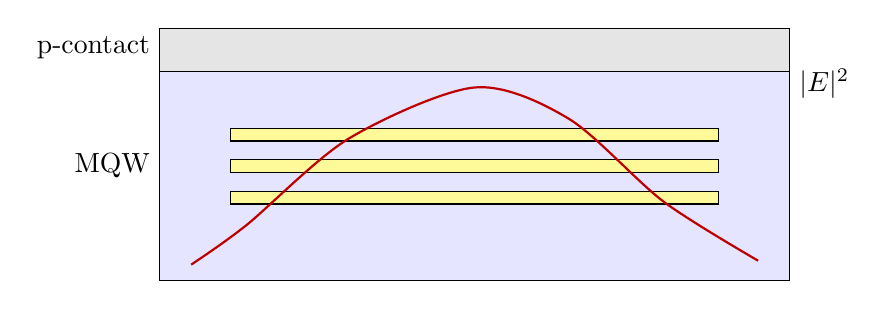
\begin{tikzpicture}[x=1cm,y=1cm]
    \draw[fill=blue!10] (0,0) rectangle (8,3.2);
    \draw[fill=gray!20] (0,2.65) rectangle (8,3.2);
    \foreach \y in {1.05,1.45,1.85} {
      \draw[fill=yellow!40] (0.9,\y-0.08) rectangle (7.1,\y+0.08);
    }
    \draw[thick,red!75!black] plot[smooth] coordinates {(0.4,0.2) (1.1,0.7) (2.4,1.8) (4.0,2.45) (5.2,2.05) (6.4,1.0) (7.6,0.25)};
    \node[left] at (0,2.95) {p-contact};
    \node[left] at (0,1.45) {MQW};
    \node[right] at (8,2.5) {$|E|^2$};
  \end{tikzpicture}
  \caption{量子阱重叠与损耗重叠示意。模式若被上表面和接触层拉得过近，即使量子阱重叠增加，也可能同时增加内部损耗。}
  \label{fig:qw-overlap}
\end{figure}

\section{掺杂和金属为什么在本章就已经是光学问题}
电注入器件需要重掺杂层和金属接触，但这不意味着它们只属于 \cref{ch:electrical}。只要模式场延伸到这些区域，它们立刻就以光学损耗的形式进入本章。工程上常用的自由载流子吸收近似可写为
\begin{equation}
\alpha_{\mathrm{fc}} \approx \sigma_n n + \sigma_p p,
\label{eq:fca_simple}
\end{equation}
其中 $n,p$ 是载流子浓度，$\sigma_n,\sigma_p$ 是等效吸收系数。\cref{eq:fca_simple} 属于\textbf{光学损耗代理模型}，它的教学意义不在于给出最精确的数值，而在于提醒读者：掺杂既改变电阻，也改变阈值。

金属的影响更不能简单理解成“再加一点吸收”。一旦模式被上拉到金属附近，不仅损耗增加，模式对称性、偏振选择与远场也会一起变化。因此，在 PCSEL 里，接触层与金属的设计不能后补。它们不是完成电学功能后再通知光学去适应，而是从一开始就应被看作光学边界条件的一部分。

\section{外延层如何改写上下辐射不对称、偏振与远场}
前面章节已经从平面内晶格的傅里叶分量和对称性角度解释了面发射、偏振与远场。但真实器件里，模式向上看到的是空气、钝化层、表面结构和金属；向下看到的是包层、衬底和更厚的半导体环境。即便平面内晶格完全对称，这种纵向边界条件的不对称也会让上、下辐射通道不等价。

这会直接影响三类量。第一是出光方向与提取效率：总辐射损耗相同，不代表向上可用的面发射功率相同。第二是偏振选择：不同矢量模与上下辐射通道的耦合权重不同，因此外延层会参与 \cref{ch:polarization} 讨论的偏振选择。第三是远场角谱：纵向相位积累和反射会改写法向附近的角分布。换句话说，\cref{ch:polarization} 那些近场-远场映射，在器件里必须与本章的纵向边界条件一起解读。

为了把这种“不对称”变成可比较的接口量，常把向上提取比例定义为
\begin{equation}
\eta_{u/d} =
\frac{P_{\mathrm{up}}}{P_{\mathrm{up}}+P_{\mathrm{down}}},
\label{eq:updown_ratio}
\end{equation}
其中 $P_{\mathrm{up}}$ 与 $P_{\mathrm{down}}$ 分别是模式向上、向下辐射的功率。\cref{eq:updown_ratio} 属于\textbf{开放光学接口量}。它不会单独决定阈值，但会直接决定“同样一支冷腔候选模”在器件里究竟是更像一个向上可用的面发射模式，还是更多地把能量泄向衬底和下包层。

\section{本章真正输出给后面三章的是什么}
到本章结束时，读者不应只得到一张层栈示意图，而应得到后面三章可直接调用的一组器件变量：目标模的纵向剖面、$\Gamma_{\mathrm{opt}}$、$\Gamma_{\mathrm{loss}}$、上下辐射不对称趋势，以及对层厚、折射率和异质结台阶变化的灵敏度。\cref{ch:qw-gain} 会把这些量与量子阱增益连接起来，\cref{ch:electrical} 会说明为什么这些外延层又决定了电流如何真正进入有源区，\cref{ch:eto-coupling} 则会展示温升如何反过来改写这些光学接口量。

这也说明了本章的真正位置：它不是器件主线的前言，而是器件主线的第一章。只要这里没有建立起来，后面关于阈值电流、模式竞争和热稳定性的讨论都只能浮在空中。

\begin{PitfallBox}
“外延层已经把量子阱放进去了，因此后续只需优化平面内晶格”是错误的。只要层厚、掺杂、金属位置或异质结台阶会改变模式的纵向位置和尾部重叠，外延层就一直在参与模式选择，而不是在几何确定后自动退出问题。
\end{PitfallBox}

\section*{本章小结}
PCSEL 的外延层首先是一个纵向光学结构，但它从一开始就带着器件物理信息进入设计。分离限制异质结构和异质结带边台阶决定了模式能否在量子阱附近取得合适重叠，同时把电子和空穴限制在可用区域；纵向层栈决定了光学约束、损耗重叠、上下辐射不对称与远场边界。有效折射率近似可以用于前期筛选，但不能取代三维器件验证。到本章结束时，读者应当已经清楚：前面章节得到的冷腔结论，只有在这里给出的外延层条件下才有机会变成真实器件结论。

\section*{练习题}
\begin{enumerate}
  \item \basicq 解释为什么 SCH 在 PCSEL 中不是可有可无的传统激光器结构，而是连接平面内光学设计与真实器件约束的基础。

  \item \basicq 结合 \cref{eq:band_offsets} 说明导带和价带台阶如何分别影响电子泄漏与空穴注入。

  \item \midq 讨论为什么增大量子阱重叠并不自动降低阈值，回答中需同时引用 $\Gamma_{\mathrm{opt}}$ 和 $\Gamma_{\mathrm{loss}}$。

  \item \hardq 给出一个你认为 effective index 近似会明显失效的 PCSEL 场景，并说明失效来自哪些纵向物理。
\end{enumerate}

\section*{建议继续阅读}
\begin{itemize}
  \item 下一章将把本章建立的异质结、量子阱和重叠语言继续推进到有源区工程，解释单量子阱、多量子阱、应变和阻挡层为什么会真正改写材料增益到模增益的映射。 这条阅读的重点是把本章的输出顺着主线接到后续模块，而不是停成孤立知识点。

  \item 若想对照一般半导体激光器中的 SCH 与波导理论，可参考 \cite{coldren2012} 中关于异质结波导、约束因子和损耗重叠的章节，但阅读时应始终记得：PCSEL 还要额外面对开放辐射与面内反馈耦合。 这条阅读的重点是补足本章关于外延层、纵向模与光学接口量 的标准背景、经典语言和代表性文献接口。

  \item 若想从器件实例反看外延层如何进入 PCSEL 主线，可参考 \cite{imada1999,hirose2014,zhoupan2023}。 这条阅读的重点是补足本章关于外延层、纵向模与光学接口量 的标准背景、经典语言和代表性文献接口。
\end{itemize}


